\clearpage
% -------------------------------------------- Benchmarks ----------------------------------------------------
\section{Benchmarks}
Over the course of the development of FluDAG a number of benchmarks were
performed, as a validation of the proof of the functionality of FluDAG the ATIC
benchmarking was performed. At the request of CERN the AlAuAl \& MagNSphere
benchmarks were performed to demonstrate the correctness for electron transport
specifically in thin geometries or near boundaries.
\label{sec:benchmarking}
\subsection{ATIC}
The Advanced Thin Ionization Calorimeter (ATIC) detector was a cosmic ray
detector flow by high altitude ballon in a number of campaigns from the year
2000 onwards. The geometry existed in a Geant4 geometry and Fluka formats, it
was decided by NASA that this geometry, shown in Figure \ref{fig:atic_geom},
would be used to validate the FluDAG code.
\begin{figure}[ht!]
 \begin{centering}
 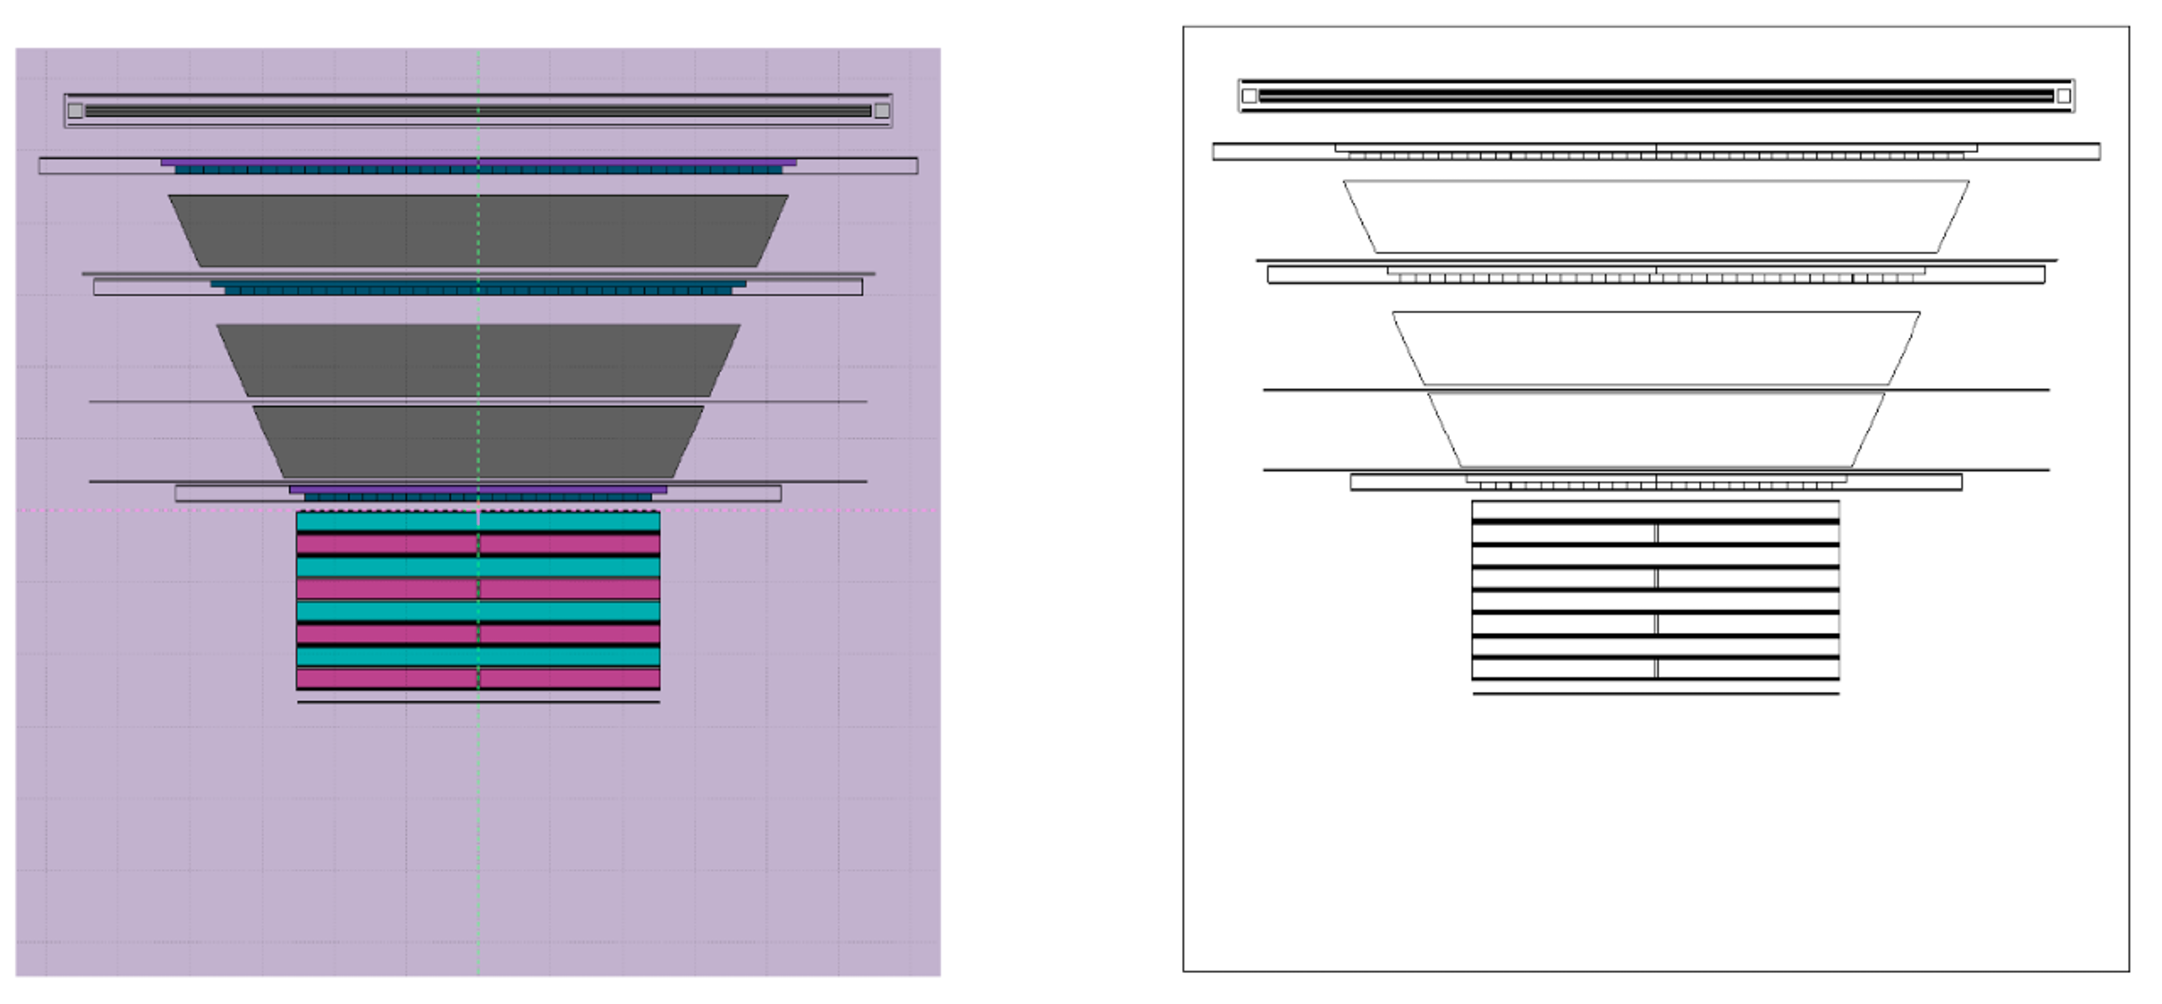
\includegraphics[width=0.7\paperwidth]{../figs/atic_geom.png}
 \caption{Geometry of the ATIC calcualtions native Fluka (left) and FluDAG (right)}
 \label{fig:atic_geom}
 \end{centering}
\end{figure}
The Fluka geometry was used as the cannonical geometry format, using Flair the
Fluka geometry was translated to MCNP format and then subsequently translated to
CAD using \texttt{mcnp2cad}. This geometry was then assigned appropriate `group
 names' for FluDAG and then faceted to produce the geometry file. This geometry
 was then used in all of the FluDAG calculations. 
\clearpage
\subsubsection*{Results}
\begin{figure}[ht!]
 \begin{centering}
 \centering
 \includegraphics[width=0.7\paperwidth]{../figs/atic_proton_flux.png}
 \caption{Proton flux profile determine in the native FLUKA geometry (left) and
          the FluDAG geometry (right)}
 \label{fig:atic_proton_flux}
 \end{centering}
\end{figure}
\begin{figure}[ht!]
 \begin{centering}
 \centering
 \includegraphics[width=0.7\paperwidth]{../figs/atic_proton_flux_lineout.png}
 \caption{Proton flux profiles, FLUKA as lines, FluDAG as points and the ratio
          of the profiles (FluDAG/Fluka)}
 \label{fig:atic_proton_flux_lineout}
 \end{centering}
\end{figure}

\begin{figure}[ht!]
 \begin{centering}
 \centering
 \includegraphics[width=0.7\paperwidth]{../figs/atic_energy_deposition.png}
 \caption{Energy deposition profile determine in the native FLUKA geometry
         (left) and the FluDAG geometry (right)}
 \label{fig:atic_energy_deposition}
 \end{centering}
\end{figure}
\begin{figure}[ht!]
 \begin{centering}
 \centering
 \includegraphics[width=0.7\paperwidth]{../figs/atic_energy_deposition_lineout.png}
 \caption{Energy deposition profiles, FLUKA as lines, FluDAG as points and the
          ratio of the profiles (FluDAG/Fluka)}
 \label{fig:atic_energy_deposition_lineout}
 \end{centering}
\end{figure}

\begin{figure}[ht!]
 \begin{centering}
 \centering
 \includegraphics[width=0.7\paperwidth]{../figs/atic_neutron_flux.png}
 \caption{Neutron flux profile determine in the native FLUKA geometry (left) and
         the FluDAG geometry (right)}
 \label{fig:atic_neutron_flux}
 \end{centering}
\end{figure}
\begin{figure}[ht!]
 \begin{centering}
 \centering
 \includegraphics[width=0.7\paperwidth]{../figs/atic_neutron_flux_lineout.png}
 \caption{Neutron flux profiles, FLUKA as lines, FluDAG as points and the ratio
         of the profiles (FluDAG/Fluka)}
 \label{fig:atic_neutron_flux_lineout}
 \end{centering}
\end{figure}

\begin{figure}[ht!]
 \begin{centering}
 \centering
 \includegraphics[width=0.7\paperwidth]{../figs/atic_photon_flux.png}
 \caption{Photon flux profile determine in the native FLUKA geometry (left)
          and the FluDAG geometry (right)}
 \label{fig:atic_photon_flux}
 \end{centering}
\end{figure}
\begin{figure}[ht!]
 \begin{centering}
 \centering
 \includegraphics[width=0.7\paperwidth]{../figs/atic_photon_flux_lineout.png}
 \caption{Photon flux profiles, FLUKA as lines, FluDAG as points and the ratio
          of the profiles (FluDAG/Fluka)}
 \label{fig:atic_photon_flux_lineout}
 \end{centering}
\end{figure}

\clearpage
\subsubsection{Conclusion}
The results shown in the previous section were shown to give excellent agreement
between Fluka \& FluDAG. For all the particles examined there was agreement
within the statistical errors with no outliers beyond 3$\sigma$. This along with
other more simplistic benchmarking activities showed that there is a direct
agreement between Fluka \& FluDAG when equivalent geometries are used. Thus
this work was presented at the 2014 Fluka Collaboration meeting and it was
agreed that this work showed sufficient merit to consider doing further
benchmarking as determined by the Fluka team.

\clearpage
\subsubsection{AlAuAl}
The AlAuAl (aluminium-gold-aluminium) benchmark originated from the development
of FLUGG. The benchmark is specifically designed to stress electron transport in
very thin layers. The geometry of the setup is shown in Figure
\ref{fig:alaual_fig}.

\begin{figure}[ht!]
 \begin{centering}
 \centering
 \includegraphics[width=0.7\paperwidth]{../figs/alaual_geom.png}
 \caption{The geometry of the setup for the AlAuAl benchmark (FLUKA geometry
         shown)}
 \label{fig:alaual_fig}
 \end{centering}
\end{figure}

The source is a 1 MeV pencil electron beam pointed in the postive z direction,
with particles starting at 0,0, -10.0 cm. The CAD model for the FluDAG was
created by exporting the native FLUKA geometry to MCNP format, then using
mcnp2cad [ref] the CAD model was created. Each calculation was run with
5.0$\times$10$^5$ with 20 batches.

\begin{figure}[ht!]
 \begin{centering}
 \centering
 \includegraphics[width=0.7\paperwidth]{../figs/alaual_spectra_lin_log.png}
 \caption{}
 \label{fig:alaual_spectra_linlog}
 \end{centering}
\end{figure}

\begin{figure}[ht!]
 \begin{centering}
 \centering
 \includegraphics[width=0.7\paperwidth]{../figs/alaual_spectra_log_log.png}
 \caption{}
 \label{fig:alaual_spectra_loglog}
 \end{centering}
\end{figure}

The suite of results displayed were shown to the FLUKA team at CERN during the
FLUKA collaboration meeting in 2015, it was agreed then that the co-oberation
between the the results are excellent and show no artifacts in the transport
of electrons. 

\clearpage
\subsubsection{Magnetic Field \& Spheres}
During the devlopment of FLUGG a specific test case gave particularly
pathogenic behaviour for electrons crossing boundaries between cells,
the test is subsequently known as MagnSph and the geometry is shown in Figure 
\ref{fig:magnsph_geom}. This test is particularly pathogenic for electron
transport due to some of the peculiarities of electron transport in general
and some of the FLUKA specific steps for electrons that are different than
other particles. The true geometry is composed of cylinders and spheres which
numerically touch. 
\\
\\
It is not possible to represent the true geometry of this benchmark in CAD
since it is not possible to resolve numerically touching, specifically with
the Cubit based workflow, ACIS can only distinguish vertices as being distinct
entities when they are greater than 1e-6 cm apart. In this instance we found
that the problem as originally defined resulted in several imprint and merge
issues. Reducing the radii of cylinder from 0.5 to 0.49999 and the radii of
the spheres from 0.3 to 0.29999 resulted in no issues regarding imprinting
or merging. However, changing the radii to 0.499999 and 0.299999 respecively
had the same issues as the unmodified model. Thus, the final model used for
the benchmark calculations were has radii of cylinders and spheres of
0.49999 and 0.29999 respectively.  

\begin{figure}[ht!]
 \begin{centering}
 \centering
 \includegraphics[width=0.7\paperwidth]{../figs/magnsph_geom.png}
 \caption{Geometry of the MagNSphe benchmark showing the incident positron source}
 \label{fig:magnsph_geom}
 \end{centering}
\end{figure}

The source is a square cross sectioned beam of side 1 cm containing positrons at 1 GeV, starting at 2,4,-1 cm directed into the postive
z direction. There is a uniform magnetic field of 60 T directed along the x direction. 

\begin{figure}[ht!]
 \begin{centering}
 \centering
 \includegraphics[width=0.9\paperwidth,angle=90]{../figs/magnsph_photon_nob.png}
 \caption{Photon flux determined in the Fluka (left) \& FluDAG (right) in the
          case without magnetic field}
 \label{fig:magnsph_photon_nob}
 \end{centering}
\end{figure}

\begin{figure}[ht!]
 \begin{centering}
 \centering
 \includegraphics[width=0.9\paperwidth,angle=90]{../figs/magnsph_electron_nob.png}
 \caption{Electron flud determined in the Fluka (left) \& FluDAG (right) in the
          case without magnetic field}
 \label{fig:magnsph_electron_nob}
 \end{centering}
\end{figure}

\begin{figure}[ht!]
 \begin{centering}
 \centering
 \includegraphics[width=0.9\paperwidth,angle=90]{../figs/magnsph_energy_nob.png}
 \caption{Energy deposition determined in the Fluka (left) \& FluDAG (right) in
          the case without magnetic field}
 \label{fig:magnsph_energy_nob}
 \end{centering}
\end{figure}

\begin{figure}[ht!]
 \begin{centering}
 \centering
 \includegraphics[width=0.9\paperwidth,angle=90]{../figs/magnsph_photon_b.png}
 \caption{Photon flux determined in the Fluka (left) \& FluDAG (right) in the
          case with magnetic fields}
 \label{fig:magnsph_photon_b}
 \end{centering}
\end{figure}

\begin{figure}[ht!]
 \begin{centering}
 \centering
 \includegraphics[width=0.9\paperwidth,angle=90]{../figs/magnsph_electron_b.png}
 \caption{Electron flux determined in the Fluka (left) \& FluDAG (right) in the
          case with magnetic fields}
 \label{fig:magnsph_electron_b}
 \end{centering}
\end{figure}

\begin{figure}[ht!]
 \begin{centering}
 \centering
 \includegraphics[width=0.9\paperwidth,angle=90]{../figs/magnsph_energy_b.png}
 \caption{Energy deposition determined in the Fluka (left) \& FluDAG (right) in
          the case with magnetic fields}
 \label{fig:magnsph_energy_b}
 \end{centering}
\end{figure}

\clearpage
